\documentclass[manuscript,linenumbers]{aastex62}

\usepackage{graphicx}
\usepackage{hyperref}
\usepackage{csvsimple}
%Use savesym to get over incompatibility with sinunitx and aastex
\usepackage{savesym}
\savesymbol{tablenum}
\usepackage{siunitx}
\restoresymbol{SIX}{tablenum}

\DeclareSIUnit[]{\jansky}{Jy}


\begin{document}

\title{RICA - Radio Imaging Combination Analyzer}
\author{Miles Lucas}
\affiliation{Iowa State University, Ames, Iowa}
\affiliation{National Radio Astronomy Observatory, Socorro, New Mexico}
 

\begin{abstract}

\end{abstract}

%---------------------------------------------------------------------------------------------------

\section{Introduction}

In radio synthesis imaging a common problem arising from interferometry is the lack of zero-spacing data. Without this data, images lack total power information. Single dish radio telescopes retain this total power information but lack the angular resolution capabilities of radio interferometers. To solve this problem, astronomers combine the interferometry data with the total power data. This report seeks to characterize the effectiveness of different combination methods and parameters.

The parameters analyzed were multiscale deconvolution versus normal Hogbom deconvolution, the effect of single-dish size on the combination, masking, and number of total iterations (i.e. depth of clean). One of the previous assumptions is that if the single-dish UV-coverage does not adequately complement the interferometer UV-coverage, feathering will not be effective. Another assumption is that simple point structures should not see much discrepancy in parameters or methods. Multiscale deconvolution is supposed to help pick up fluffy structure better due to its multi-pass method of creating model images in the Cotton-Schwab Cycle, as opposed to Hogbom's $\delta$-function method. Therefore, more complex, fluffy structure ought to show more distinction in results.

There are four methods of combination that were tested. The first is CASA's \textit{feather} task. The process of feathering starts with regridding the lower resolution to the higher resolution image. Each is then Fourier transformed and gridded, while the lower resolution data is scaled by the ratio of the clean beams (high resolution/low resolution). The high-resolution grid is then added to this, scaled by a weighting that starts at 0 and increases to 1 as the wavelength increases. This final combination is then inverse Fourier transformed back into the image plane. 

The next method is using the total power image as the starting model in CASA's \textit{tclean} task. In the Cotton-Schwab CLEAN algorithm (CSCLEAN), each major-cycle begins with a blank model image and constructs an image on it by using minor-cycle iterations. By using a starting model, this model is no longer blank, but is passed as a parameter. By using the total power image as the starting model, we can hope to retain the total power information through the CLEAN algorithm.

Another modification to the Cotton-Schwab cycle in order to combine images is by doing a modified joint deconvolution. In each major Cotton-Schwab cycle, the visibilities are gridded and inverse Fourier transformed to create an image residual, which is then feathered with the total power residual before deconvolving. The deconvolved model is then convolved with the single-dish beam and subtracted from the previous single-dish residual. The deconvolved model is also Fourier transformed, degridded, and subtracted from the visibilities to create a new residual image These residuals are then degridded and transformed to finish the major cycle. See \autoref{fig:jd-flow} for a visual flowchart of the process.

\begin{figure*}[t]
    \plotone{figures/joint-deconvolve}
    \caption{A flow chart describing the joint-deconvolution approach to combining interferometer and single dish data. Adapted from Rau, U. \& Naik, N. 2018 (in prep).}
    \label{fig:jd-flow}
\end{figure*}

The last method of combination we use is \textit{tp2vis}, which takes the total power image and spoofs a measurement set. The way \textit{tp2vis} accomplishes this is by taking Fourier data from the total power image and sparsely sampling the Fourier data at close spacings \citep[see][]{2011ApJS..193...19K}. This data can be concatenated with the interferometer data and deconvolved in \textit{tclean}. \autoref{fig:tp2vis} shows how the single-dish is simulated and concatenated with the interferometer data. This should help fill the close-spacing gap created by the interferometer data and subsequently help increase total power information.

\begin{figure*}[t]
    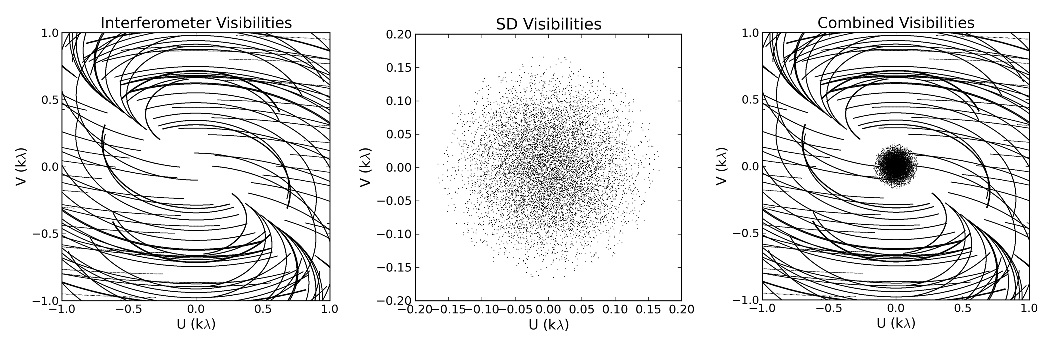
\includegraphics[width=\textwidth]{figures/tp2vis}
    \caption{A look at how the visibilities are added through using tp2vis for a model simulated on the VLA A configuration. In the center of the interferometer image in the first plot shows sparsity that is filled in on the third plot. The second plot shows the approximation tp2vis makes of the single dish.}
    \label{fig:tp2vis}
\end{figure*}

%---------------------------------------------------------------------------------------------------

\section{Methods}

In order to evaluate the different combination methods, a metric needed to be created and tested on a suite of models. The metrics used were CLEAN residuals, fidelity images, and a ratio of the power spectrum densities (PSD). The fidelities are given \autoref{eqn:fidelity} 
 
\begin{equation}
    \text{Fidelity}(i, j) = \frac{|\text{Model}(i, j)|}{\max{\left(|\text{Difference}(i, j)|, 0.7\times\text{rms}(\text{Difference})\right)}}
    \label{eqn:fidelity}
\end{equation} 

where model is the reference image and diff is the difference between the test and reference images \citep[p.19]{almamemo}. The exigence for using PSDs is that the zero-spacing power is readily visible for every image. By using these ratios, the closer the ratio is to 1.0 at short spacings (when compared to the true model), the more accurate the combination. In addition, when compared with the total power image, it shows how much effective weight is given to the total power image in the combination. The ratio of the PSDs is given by \autoref{eqn:ratio}

\begin{equation}
    \text{Ratio}(UV) = \frac{\text{Power}_{test}(UV)}{\text{Power}_{ref}(UV)} \cdot \frac{\text{BA}_{ref}}{\text{BA}_{test}}
    \label{eqn:ratio}
\end{equation} 

\begin{equation}
    \text{err}(UV) = \left(\frac{\text{Power}_{ref}(UV)+ \text{Power}_{test}(UV)}{2}\right)^{-1}
    \label{eqn:ratio-err}
\end{equation} 

where Power is the power from the PSD, BA is the beam area, $ref$ refers to the reference image (model or SD), and $test$ refers to whichever image is being tested. The uncertainty given is \autoref{eqn:ratio-err} such that the uncertainty is the reciprocal of the average of the PSDs. 

Each combination was compared to both the true model and the single dish, total power image. Many models were tested with various extra parameters. Three models were generated from component lists. One has 4 point sources, one has a single Gaussian source, and one has a mixture of 4 point sources, one very broad Gaussian, and on off-center, stronger Gaussian. There were also various models based off real structure, including M51 (based off an H-$\alpha$ image), Orion, RXJ1347, which is a source displaying the Sunyaev-Zel'dovich effect \citep{2016PASJ...68...88K}, and a protoplanetary disk (PPD) simulation. \autoref{fig:models} shows all of the models. It is important to note that these models have been regridded onto a common coordinate system that is not representative of the true astronomical targets. This was in effort to simplify the simulation process for creating measurement sets. 

\begin{figure*}[t]
    \includegraphics[width=\textwidth]{figures/models}
    \caption{The models used for testing combination methods convolved with some restoring beam to show structure better.}
    \label{fig:models}
\end{figure*}

The code base for testing the effectiveness is hosted publicly for anyone to use\footnote{\url{https://gitlab.com/mileslucas/rica}}. In the source code there are many scripts and methods to facilitate simulating, combining, and comparing. Every model is described in \textit{src/\_models.py} with a dictionary defining the simulation and \textit{tclean} parameters. The pipeline for testing these models was as follows:
\begin{enumerate}
    \item Simulate measurement set (MS) based on VLA configurations
    \item Simulate single dish image by convolving model with Gaussian
    \item Image the MS 
    \item Do the combinations (feather, startmodel, joint deconvolution, and tp2vis)
    \item For each combination, do a comparison with the true model (convolved with the restoring beam) and the single dish image
\end{enumerate}
and is implemented in \textit{src/pipeline.py}. 

\subsection{Simulations and Deconvolution}
All simulations were done using the VLA for the telescope model except for the PPD simulation, which was done using \textit{simalma}. Each test model could define which of the VLA configurations to use, from A, B, BnA, C, CnB, D, and DnC. The spectral window for the simulations mimic the VLA C-band at \SIrange{4.5}{5.5}{\giga\hertz} (central \SI{5}{\giga\hertz}) with 101 channels at \SI{10}{\mega\hertz} intervals. The field observed was J2000 21h28m31.0 \ang{45;00;00.0}. The observation date and time was 2018/06/01 at 12:00:00.0 UTC. The integration time was \SI{10}{\second} each with a total of \SI{30000}{\second}. Finally, the data was corrupted with \SI{1}{\milli\jansky} of simple noise.

The PPD model was created by following the \href{https://casaguides.nrao.edu/index.php/Protoplanetary_Disk_Simulation_(CASA_5.1)}{CASA guide for simulation}. The base model is from \citet{2005ApJ...619.1114W}, which is a simulation of ALMA data at \SI{672}{\giga\hertz}. This involved one pointing at J2000 18h00m00.031s -22d59m59.6s observed for \SI{20}{\minute} in the ALMA configuration 20. The total power image was created using \textit{simalma} to recreate the Atacama Compact Array (ACA) with its \SI{12}{\meter} single dish telescopes. 

The single dish images were created by taking the true model and convolving with a Gaussian equivalent to the single dish beam at the given frequency. 
\begin{equation}
    \text{FWHM}(\nu, D) = \frac{\SI{3.66e8}{\meter\per\second}}{\nu \cdot D}
    \label{eqn:sdbeam}
\end{equation}
\autoref{eqn:sdbeam} gives the Gaussian kernel full-width half-maximum (FWHM) in radians for a frequency in Hz and dish diameter in meters. For instance, to simulate data from the Green Bank Telescope (GBT) with a dish diameter of \SI{100}{\meter} at \SI{5}{\giga\hertz} gives a FWHM of \ang{;2;31}, which is in agreeance with values from the GBT proposer's guide\footnote{p.9, \url{https://science.nrao.edu/facilities/gbt/proposing/GBTpg.pdf}}. Note that this is not the most accurate equation for other telescopes, because there is a constant involved in this equation based off the taper-length of the telescope's feedhorns. In addition, these single dish images have \num{5e-6} uniform noise added. 

Each model defines its own parameters for cleaning. \autoref{tab:model-params} lists every single parameter for each model. As a default, a model simulated in VLA D configuration has an image size of \num{64} with a cell size of \SI{7.0}{\arcsec}. The restoring beam for the D configuration is approximately \ang{;;20.41} by \ang{;;15.60} so the cell accounts for half to a third of the beam width. In general, cleaning was done with very high numbers of iterations, relying on a threshold to stop the algorithm for consistency. This differs for the models tested at explicitly different cleaned levels.



\subsection{Comparisons}
Each comparison was ran with the same clean parameters for consistency. Because \textit{feather} does not actively clean, it has its own set of parameters, but all of the models tested used the default parameters. After all the combination permutations were imaged, they were compared against the true model convolved with the restoring beam and the single dish image alongside the uncombined interferometer image. All of the ratio were saved into individual CSV files for further analysis. In all, each model has 10 comparisons (5 against the models and 5 against the single-dish images) and 4 separate cleans to perform. 

In order to run a new model to test comparison methods, there are two general methods. If there exists a true model, simply add an entry to the models dictionary defining the simulation and clean parameters. It is also important to edit \textit{src/simulate.py} to accommodate the new model. Follow the existing code base for guidance. It is also important to create a copy of the model and regrid it to the common coordinate system (use an existing model to retrieve the coordinate system). The model can then be ran through the pipeline along with any other models using \textit{src/pipeline.py}.

If there is no true model, it is still useful to test and compare against the total power image, alone. In this case, using a cleaned image, a measurement set, and a total power image with the \textit{src/combine.py} script will produce all of the combinations. These can then be compared using \textit{src/compare.py}. It is possible to edit \textit{src/pipeline.py} to accommodate special models, see how the PPD model is handled in the pipeline. 




%---------------------------------------------------------------------------------------------------

\section{Results}

\begin{figure*}[ht]
    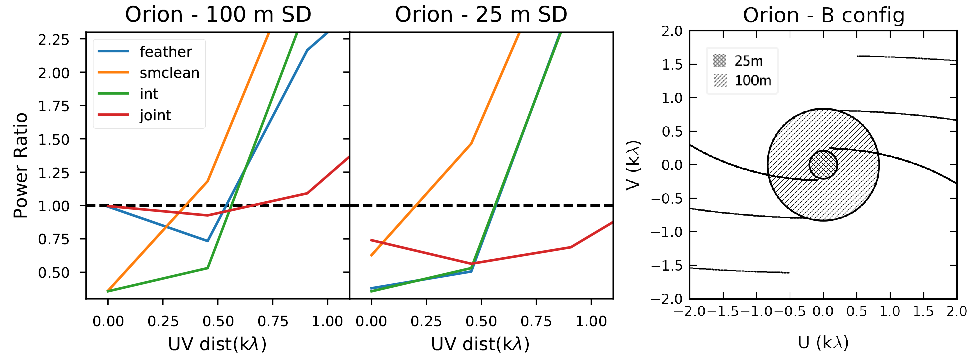
\includegraphics[width=\textwidth]{figures/sd_size_comp}
    \caption{The left two plots are ratios for each combination method between two different single dish sizes. The horizontal line marks the ideal ratio for close UV spacing. The right plot shows the UV coverage of the interferometer with the coverage of the \SI{100}{\meter} and \SI{25}{\meter} single dishes overlaid.}
    \label{fig:sd-size}
\end{figure*}

For fidelity images and ratios of every comparison, see \autoref{sec:model-results}. This section will only comment on a few models and comparison highlighting trends. The effect of single dish size was apparent on the accuracy of combinations. \autoref{fig:sd-size} shows how the ratios compare between the \SI{100}{\meter} single dish size for the Orion model in B configuration and the \SI{25}{\meter} single dish size of the same model. Notably, \textit{feather} does not work as well for small single dish sizes. Both start model and joint deconvolution combination methods are able to do better than the plain interferometer with the small dish, but still do not reach that ideal ratio that is possible for the larger single dish. Looking at the coverage of the single dishes, the \SI{25}{\meter} dish does not overlap with the interferometer data at all.

\begin{figure*}[ht]
    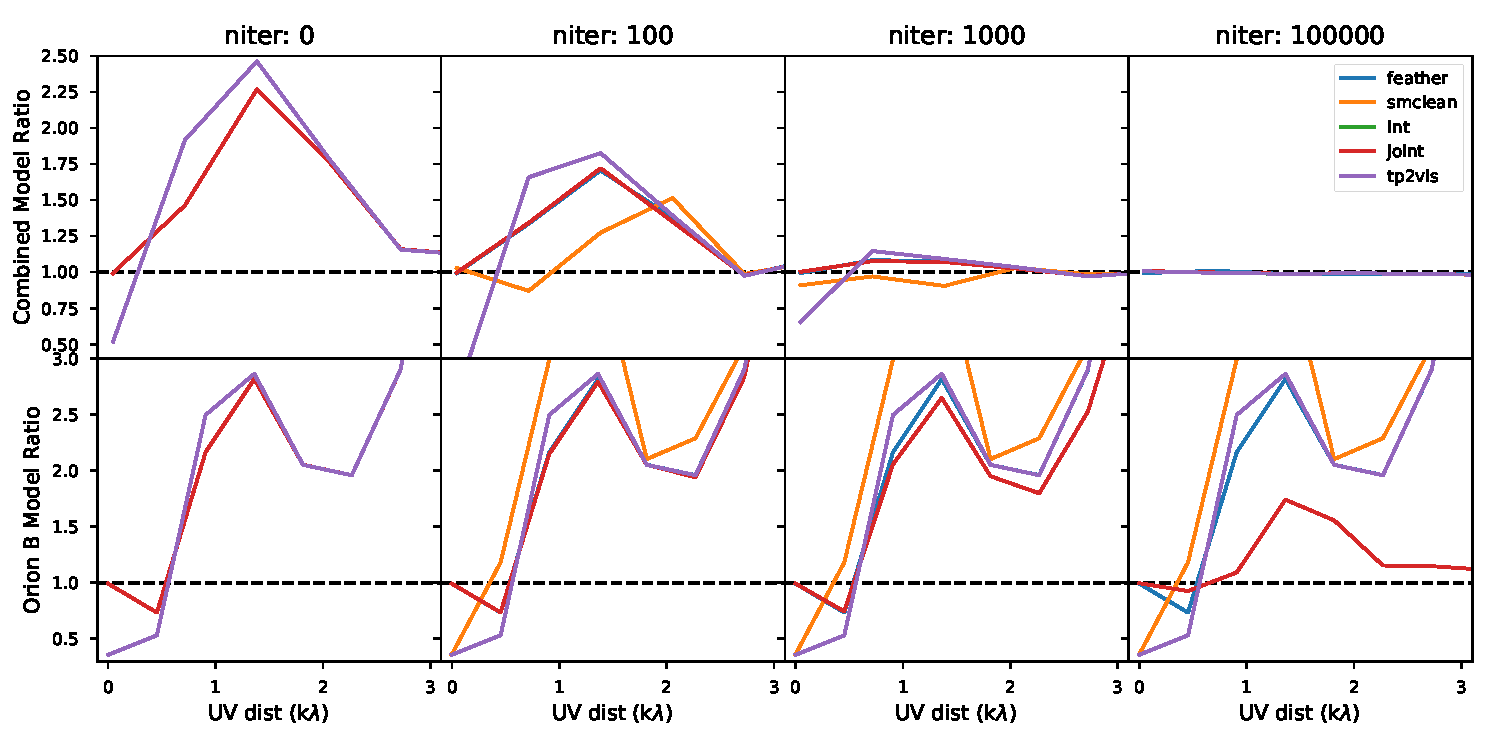
\includegraphics[width=\textwidth]{figures/iter-plot}
    \caption{A comparison showing the effect on the combinations due to the depth of cleaning for two models, `combined' and `orion-b'. The dashed black line represents the ideal ratio for the true model comparison. }
    \label{fig:iters}
\end{figure*}

Next, \autoref{fig:iters} shows the effect that depth of cleaning has on the power ratios. Each row corresponds to each model and each column is a depth of cleaning based on the number of iterations of deconvolution. The `combined' model is a much simpler model than the `orion-b' model. First, the joint deconvolution worked well regardless of the depth of cleaning for both models. Even completely dirty images had great total power information. After some amount of cleaning, \textit{feather} quickly rose to the same level as joint deconvolution and in the `combined' model, using a start model started working after some cleaning. In the simpler, `combined' model, all combination methods converged at high enough iterations- even the interferometer image. However, for the more complex, `orion-b' model, start model never converged and the values of the ratios remained erratic even at full cleaning depth.

\begin{figure*}[ht]
    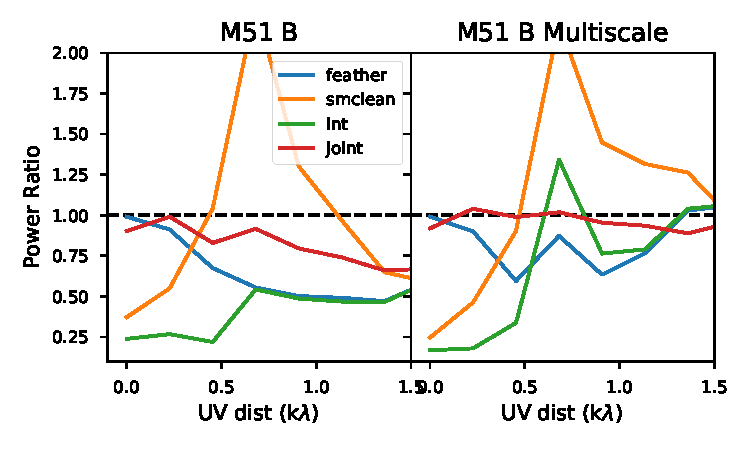
\includegraphics[width=0.49\textwidth]{figures/M51-B-Multiscale}
    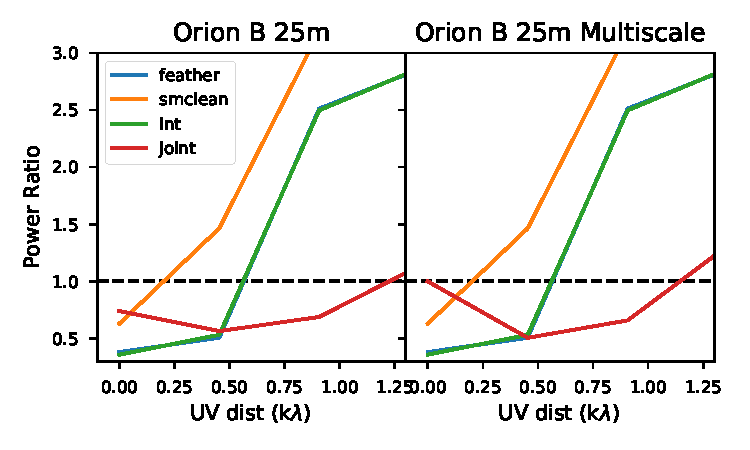
\includegraphics[width=0.49\textwidth]{figures/Orion-B-25m-Multiscale}
    \caption{A comparison showing the effect on the combinations due to multiscale deconvolution for two models, `m51-b' and `orion-b'. The dashed black line represents the ideal ratio for the true model comparison. }
    \label{fig:ms}
\end{figure*}

\autoref{fig:ms} shows how multiscale deconvolution affects the combinations. For each model, there are some slight variations, but in general the ratios stay consistent. The `orion-b-25' multiscale model shows how multiscale can improve efficiency for joint deconvolution when the single dish overlap is low. The `orion-b' multiscale model (not shown) does not show much change between deconvolvers except for an unexplained overshoot in the multiscale joint deconvolution.

\begin{figure*}[ht]
    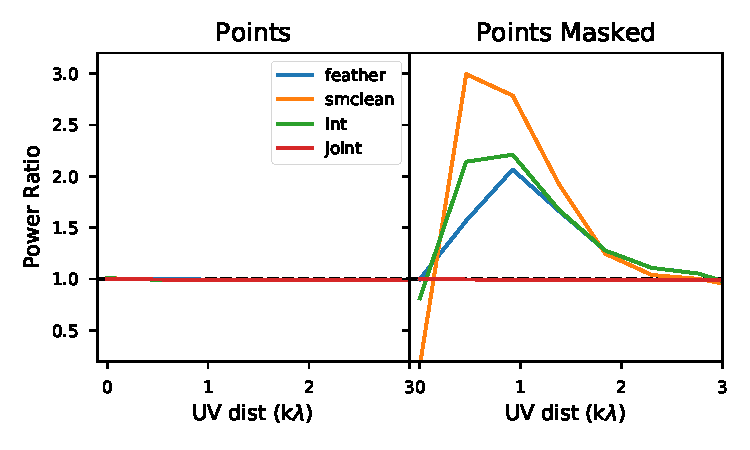
\includegraphics[width=0.49\textwidth]{figures/Points-Masked}
    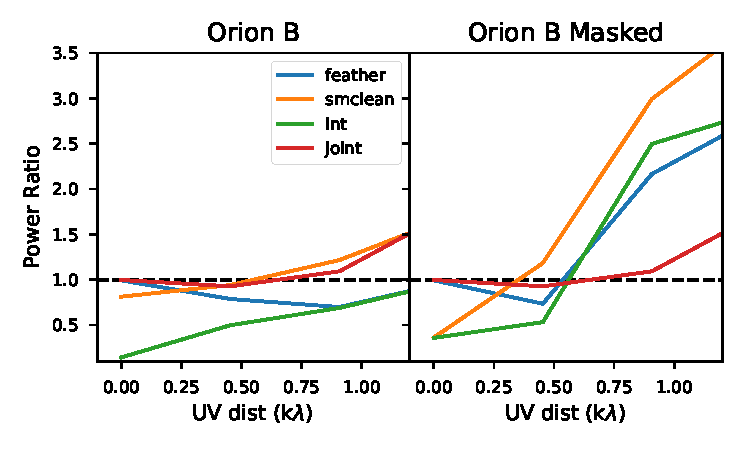
\includegraphics[width=0.49\textwidth]{figures/Orion-B-Masked}
    \caption{A comparison showing the effect on the combinations due to masking for two models, `points' and `orion-b'. The dashed black line represents the ideal ratio for the true model comparison. }
    \label{fig:masked}
\end{figure*}

\autoref{fig:masked} shows the effect masking has on the combinations. For the simple `points' model masking causes issues, especially with startmodel. Also, in the `orion-b' model, the startmodel value falls at \num{0} UV spacing, as well as the plain, cleaned image. In general, the masking decreases the convergence of the combination methods at the same clean level and may have further affects by changing the performance of the uncombined image. This is also apparent in the `RXJ1347' masked model, where the \num{0} UV spacing value does not change but the convergence is definitely affected.


\begin{figure*}[ht]
    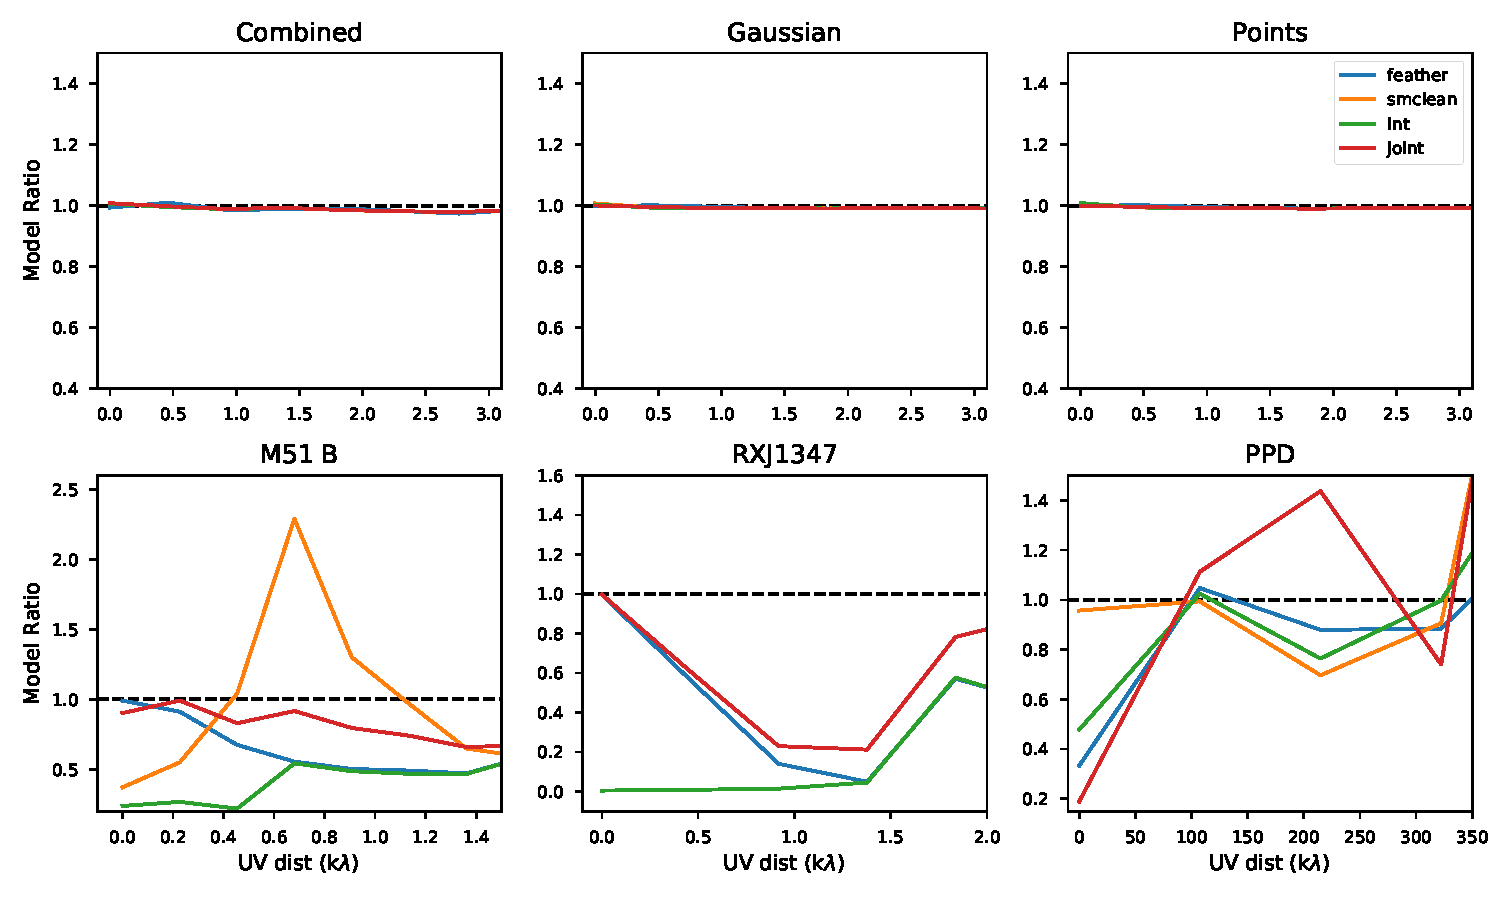
\includegraphics[width=\textwidth]{figures/complexity-plot}
    \caption{A comparison of many models. The top row are `simple' models that do not contain much structure or extended emission, whereas the second row contains more complex models with different structural scales and interesting phenomenon (Sunyaev-–Zel'dovich effect in RXJ1347).}
    \label{fig:complex}
\end{figure*}

\autoref{fig:complex} shows an overview of the performance of different models. Simpler models with point sources and Gaussians converge at a ratio of \num{1} and show very little difference until scales at hundredths of a ratio. The more complex models have no easy, clear trend. Each one of these combinations is highly dependent on the structure and parameters. It is interesting that the ALMA `PPD' model only performs well with startmodel and that \textit{feather} and joint deconvolution actually perform worse than the uncombined image. 
%---------------------------------------------------------------------------------------------------

\section{Conclusion}

From the results of the single dish sizes, the main factor in algorithm success is the amount of overlap of the single dish and interferometer data. This could be the reason why feather fails so much and why joint deconvolution and start model are not quite as good, either. Future studies might find the point at which there is enough overlay for each method to ``succeed". 

In regards to the depth of cleaning, in general, more is better. Joint deconvolution seemed to work for any dirty image with enough single dish coverage, but for future studies, it would be nice to try and see if joint deconvolution works for dirty images of many more models. In conjunction with the study on single dish size, there were no combinations that retrieved the total power information well from the dirty image due to insufficient single dish coverage\footnote{see \href{https://gitlab.com/mileslucas/rica/blob/master/docs/static/ratios/orion-b-25-n0__model.csv}{'orion-b-25-n0' ratio data}}

The multiscale analysis shows that using the multiscale deconvolver can make up for lack of single dish UV coverage in some instances. When there is already decent 



%---------------------------------------------------------------------------------------------------

\acknowledgments
Thank you to Dr. Kumar Golap and Dr. Takahiro Tsutsumi for their guidance and assistance. This work was funded by the National Science Foundation in partnership with the National Radio Astronomy Observatory and Associated Universities Incorporated.

\software{\href{https://casa.nrao.edu}{CASA}, \href{https://github.com/tp2vis/distribute}{tp2vis} \citep{2011ApJS..193...19K}}

\bibliography{sources}

\appendix
\section{Model Parameters}
\label{sec:models}

The following table describes the parameters used for cleaning the model images. The only exception is the model `combined-sp', which additionally uses specmode='cube' and nchan=-1 to facilitate cube imaging. For more details, look at the \textit{src/\_models.py} file, which this table is generated from.
\begin{longrotatetable}
    
    \label{tab:model-params}
    \begin{deluxetable}{cccllllllclc}
        \tablecaption{The parameters for every model ran through the pipeline}
        \tablehead{
        \colhead{Name} & \colhead{Model} &	\colhead{Config} &	\colhead{SD size} &	\colhead{imsize} &	\colhead{cell} &	\colhead{niter} &	\colhead{cycleniter} &	\colhead{threshold} &	\colhead{deconvolver} & \colhead{scales} & \colhead{mask} \\
        }
        
        \startdata
        points & points & VLA d & 100 m & [64, 64] & 7.00arcsec & 100000 & 100 & 1e-5Jy & hogbom &  & No \\
points-masked & points & VLA d & 100 m & [64, 64] & 7.00arcsec & 100000 & 100 & 1e-5Jy & hogbom &  & Yes \\
gauss & gauss & VLA d & 100 m & [64, 64] & 7.00arcsec & 100000 & 100 & 1e-5Jy & hogbom &  & No \\
combined & combined & VLA d & 100 m & [64, 64] & 7.00arcsec & 100000 & 100 & 1e-5Jy & hogbom &  & No \\
combined-sp & combined & VLA d & 100 m & [64, 64] & 7.00arcsec & 100000 & 100 & 1e-5Jy & hogbom &  & No \\
combined-n0 & combined & VLA d & 100 m & [64, 64] & 7.00arcsec & 0 & 100 & 1e-5Jy & hogbom &  & No \\
combined-n100 & combined & VLA d & 100 m & [64, 64] & 7.00arcsec & 100 & 100 & 1e-5Jy & hogbom &  & No \\
combined-n1000 & combined & VLA d & 100 m & [64, 64] & 7.00arcsec & 1000 & 100 & 1e-5Jy & hogbom &  & No \\
combined-ms & combined & VLA d & 100 m & [64, 64] & 7.00arcsec & 100000 & 100 & 1e-5Jy & multiscale & [0, 3, 10, 30] & No \\
m51 & m51 & VLA d & 100 m & [128, 128] & 7.00arcsec & 100000 & 100 & 1e-12Jy & hogbom &  & No \\
m51-ms & m51 & VLA d & 100 m & [128, 128] & 7.00arcsec & 100000 & 100 & 1e-12Jy & multiscale & [0, 3, 10, 30] & No \\
m51-b & m51 & VLA b & 100 m & [1400, 1400] & 0.65arcsec & 100000 & 100 & 1e-12Jy & hogbom &  & No \\
m51-b-ms & m51 & VLA b & 100 m & [1400, 1400] & 0.65arcsec & 100000 & 100 & 1e-12Jy & multiscale & [0, 3, 10, 30] & No \\
orion-b-unmasked & orion & VLA b & 100 m & [700, 700] & 0.65arcsec & 100000 & 400 & 1e-9Jy & hogbom &  & No \\
orion-b & orion & VLA b & 100 m & [700, 700] & 0.65arcsec & 100000 & 400 & 1e-9Jy & hogbom &  & Yes \\
orion-b-n0 & orion & VLA b & 100 m & [700, 700] & 0.65arcsec & 0 & 100 & 1e-9Jy & hogbom &  & Yes \\
orion-b-n100 & orion & VLA b & 100 m & [700, 700] & 0.65arcsec & 100 & 100 & 1e-9Jy & hogbom &  & Yes \\
orion-b-n1000 & orion & VLA b & 100 m & [700, 700] & 0.65arcsec & 1000 & 100 & 1e-9Jy & hogbom &  & Yes \\
orion-b-ms & orion & VLA b & 100 m & [700, 700] & 0.65arcsec & 100000 & 400 & 1e-9Jy & multiscale & [0, 3, 10, 50] & Yes \\
orion-b-25 & orion & VLA b & 25 m & [700, 700] & 0.65arcsec & 100000 & 400 & 1e-9Jy & hogbom &  & Yes \\
orion-b-25-n0 & orion & VLA b & 25 m & [700, 700] & 0.65arcsec & 0 & 100 & 1e-9Jy & hogbom &  & Yes \\
orion-b-25-n100 & orion & VLA b & 25 m & [700, 700] & 0.65arcsec & 100 & 100 & 1e-9Jy & hogbom &  & Yes \\
orion-b-25-n1000 & orion & VLA b & 25 m & [700, 700] & 0.65arcsec & 1000 & 100 & 1e-9Jy & hogbom &  & Yes \\
orion-b-25-ms & orion & VLA b & 25 m & [700, 700] & 0.65arcsec & 100000 & 400 & 1e-9Jy & multiscale & [0, 3, 10, 30] & Yes \\
orion-c & orion & VLA c & 100 m & [216, 216] & 2.12arcsec & 100000 & 400 & 1e-9Jy & hogbom &  & No \\
RXJ1347 & RXJ1347 & VLA a & 100 m & [2268, 2268] & 0.20arcsec & 100000 & 100 & 1e-6Jy & hogbom &  & No \\
RXJ1347-masked & RXJ1347 & VLA a & 100 m & [2268, 2268] & 0.20arcsec & 100000 & 100 & 1e-6Jy & hogbom &  & Yes \\
ppd & ppd & ALMA 20 & 12 m & [192, 192] & 0.01arcsec & 100000 & 100 & 1e-7Jy & hogbom &  & No 

        \enddata
        \end{deluxetable}
\end{longrotatetable}

\section{Model Results}
\label{sec:model-results}

For data tables of every single comparison, visit the \href{https://gitlab.com/mileslucas/rica/tree/master/docs/static/ratios}{RICA repository}.

\figsetstart
\figsetnum{1}
\figsettitle{Model Results}

\figsetgrpstart
\figsetgrpnum{1.1}
\figsetgrptitle{combined-ms}
\figsetplot{figures/results/combined-ms__model_vs_feather.png}
\figsetplot{figures/results/combined-ms__model_vs_int.png}
\figsetplot{figures/results/combined-ms__model_vs_joint.png}
\figsetplot{figures/results/combined-ms__model_vs_smclean.png}
\figsetplot{figures/results/combined-ms__model_vs_tp2vis.png}
\figsetgrpnote{The comparison for feather combination to the true model.}
\figsetgrpend

\figsetgrpstart
\figsetgrpnum{1.2}
\figsetgrptitle{combined-n0}
\figsetplot{figures/results/combined-n0__model_vs_feather.png}
\figsetplot{figures/results/combined-n0__model_vs_int.png}
\figsetplot{figures/results/combined-n0__model_vs_joint.png}
\figsetplot{figures/results/combined-n0__model_vs_smclean.png}
\figsetplot{figures/results/combined-n0__model_vs_tp2vis.png}
\figsetgrpnote{The comparison for feather combination to the true model.}
\figsetgrpend

\figsetgrpstart
\figsetgrpnum{1.3}
\figsetgrptitle{combined-n1000}
\figsetplot{figures/results/combined-n1000__model_vs_feather.png}
\figsetplot{figures/results/combined-n1000__model_vs_int.png}
\figsetplot{figures/results/combined-n1000__model_vs_joint.png}
\figsetplot{figures/results/combined-n1000__model_vs_smclean.png}
\figsetplot{figures/results/combined-n1000__model_vs_tp2vis.png}
\figsetgrpnote{The comparison for feather combination to the true model.}
\figsetgrpend

\figsetgrpstart
\figsetgrpnum{1.4}
\figsetgrptitle{combined-n100}
\figsetplot{figures/results/combined-n100__model_vs_feather.png}
\figsetplot{figures/results/combined-n100__model_vs_int.png}
\figsetplot{figures/results/combined-n100__model_vs_joint.png}
\figsetplot{figures/results/combined-n100__model_vs_smclean.png}
\figsetplot{figures/results/combined-n100__model_vs_tp2vis.png}
\figsetgrpnote{The comparison for feather combination to the true model.}
\figsetgrpend

\figsetgrpstart
\figsetgrpnum{1.5}
\figsetgrptitle{combined}
\figsetplot{figures/results/combined__model_vs_feather.png}
\figsetplot{figures/results/combined__model_vs_int.png}
\figsetplot{figures/results/combined__model_vs_joint.png}
\figsetplot{figures/results/combined__model_vs_smclean.png}
\figsetplot{figures/results/combined__model_vs_tp2vis.png}
\figsetgrpnote{The comparison for feather combination to the true model.}
\figsetgrpend

\figsetgrpstart
\figsetgrpnum{1.6}
\figsetgrptitle{gauss}
\figsetplot{figures/results/gauss__model_vs_feather.png}
\figsetplot{figures/results/gauss__model_vs_int.png}
\figsetplot{figures/results/gauss__model_vs_joint.png}
\figsetplot{figures/results/gauss__model_vs_smclean.png}
\figsetplot{figures/results/gauss__model_vs_tp2vis.png}
\figsetgrpnote{The comparison for feather combination to the true model.}
\figsetgrpend

\figsetgrpstart
\figsetgrpnum{1.7}
\figsetgrptitle{m51-b-ms}
\figsetplot{figures/results/m51-b-ms__model_vs_feather.png}
\figsetplot{figures/results/m51-b-ms__model_vs_int.png}
\figsetplot{figures/results/m51-b-ms__model_vs_joint.png}
\figsetplot{figures/results/m51-b-ms__model_vs_smclean.png}
\figsetplot{figures/results/m51-b-ms__model_vs_tp2vis.png}
\figsetgrpnote{The comparison for feather combination to the true model.}
\figsetgrpend

\figsetgrpstart
\figsetgrpnum{1.8}
\figsetgrptitle{m51-b}
\figsetplot{figures/results/m51-b__model_vs_feather.png}
\figsetplot{figures/results/m51-b__model_vs_int.png}
\figsetplot{figures/results/m51-b__model_vs_joint.png}
\figsetplot{figures/results/m51-b__model_vs_smclean.png}
\figsetplot{figures/results/m51-b__model_vs_tp2vis.png}
\figsetgrpnote{The comparison for feather combination to the true model.}
\figsetgrpend

\figsetgrpstart
\figsetgrpnum{1.9}
\figsetgrptitle{m51-ms}
\figsetplot{figures/results/m51-ms__model_vs_feather.png}
\figsetplot{figures/results/m51-ms__model_vs_int.png}
\figsetplot{figures/results/m51-ms__model_vs_joint.png}
\figsetplot{figures/results/m51-ms__model_vs_smclean.png}
\figsetplot{figures/results/m51-ms__model_vs_tp2vis.png}
\figsetgrpnote{The comparison for feather combination to the true model.}
\figsetgrpend

\figsetgrpstart
\figsetgrpnum{1.10}
\figsetgrptitle{m51}
\figsetplot{figures/results/m51__model_vs_feather.png}
\figsetplot{figures/results/m51__model_vs_int.png}
\figsetplot{figures/results/m51__model_vs_joint.png}
\figsetplot{figures/results/m51__model_vs_smclean.png}
\figsetplot{figures/results/m51__model_vs_tp2vis.png}
\figsetgrpnote{The comparison for feather combination to the true model.}
\figsetgrpend

\figsetgrpstart
\figsetgrpnum{1.11}
\figsetgrptitle{orion-b-25-ms}
\figsetplot{figures/results/orion-b-25-ms__model_vs_feather.png}
\figsetplot{figures/results/orion-b-25-ms__model_vs_int.png}
\figsetplot{figures/results/orion-b-25-ms__model_vs_joint.png}
\figsetplot{figures/results/orion-b-25-ms__model_vs_smclean.png}
\figsetplot{figures/results/orion-b-25-ms__model_vs_tp2vis.png}
\figsetgrpnote{The comparison for feather combination to the true model.}
\figsetgrpend

\figsetgrpstart
\figsetgrpnum{1.12}
\figsetgrptitle{orion-b-25-n0}
\figsetplot{figures/results/orion-b-25-n0__model_vs_feather.png}
\figsetplot{figures/results/orion-b-25-n0__model_vs_int.png}
\figsetplot{figures/results/orion-b-25-n0__model_vs_joint.png}
\figsetplot{figures/results/orion-b-25-n0__model_vs_smclean.png}
\figsetplot{figures/results/orion-b-25-n0__model_vs_tp2vis.png}
\figsetgrpnote{The comparison for feather combination to the true model.}
\figsetgrpend

\figsetgrpstart
\figsetgrpnum{1.13}
\figsetgrptitle{orion-b-25-n1000}
\figsetplot{figures/results/orion-b-25-n1000__model_vs_feather.png}
\figsetplot{figures/results/orion-b-25-n1000__model_vs_int.png}
\figsetplot{figures/results/orion-b-25-n1000__model_vs_joint.png}
\figsetplot{figures/results/orion-b-25-n1000__model_vs_smclean.png}
\figsetplot{figures/results/orion-b-25-n1000__model_vs_tp2vis.png}
\figsetgrpnote{The comparison for feather combination to the true model.}
\figsetgrpend

\figsetgrpstart
\figsetgrpnum{1.14}
\figsetgrptitle{orion-b-25-n100}
\figsetplot{figures/results/orion-b-25-n100__model_vs_feather.png}
\figsetplot{figures/results/orion-b-25-n100__model_vs_int.png}
\figsetplot{figures/results/orion-b-25-n100__model_vs_joint.png}
\figsetplot{figures/results/orion-b-25-n100__model_vs_smclean.png}
\figsetplot{figures/results/orion-b-25-n100__model_vs_tp2vis.png}
\figsetgrpnote{The comparison for feather combination to the true model.}
\figsetgrpend

\figsetgrpstart
\figsetgrpnum{1.15}
\figsetgrptitle{orion-b-25}
\figsetplot{figures/results/orion-b-25__model_vs_feather.png}
\figsetplot{figures/results/orion-b-25__model_vs_int.png}
\figsetplot{figures/results/orion-b-25__model_vs_joint.png}
\figsetplot{figures/results/orion-b-25__model_vs_smclean.png}
\figsetplot{figures/results/orion-b-25__model_vs_tp2vis.png}
\figsetgrpnote{The comparison for feather combination to the true model.}
\figsetgrpend

\figsetgrpstart
\figsetgrpnum{1.16}
\figsetgrptitle{orion-b-ms}
\figsetplot{figures/results/orion-b-ms__model_vs_feather.png}
\figsetplot{figures/results/orion-b-ms__model_vs_int.png}
\figsetplot{figures/results/orion-b-ms__model_vs_joint.png}
\figsetplot{figures/results/orion-b-ms__model_vs_smclean.png}
\figsetplot{figures/results/orion-b-ms__model_vs_tp2vis.png}
\figsetgrpnote{The comparison for feather combination to the true model.}
\figsetgrpend

\figsetgrpstart
\figsetgrpnum{1.17}
\figsetgrptitle{orion-b-n0}
\figsetplot{figures/results/orion-b-n0__model_vs_feather.png}
\figsetplot{figures/results/orion-b-n0__model_vs_int.png}
\figsetplot{figures/results/orion-b-n0__model_vs_joint.png}
\figsetplot{figures/results/orion-b-n0__model_vs_smclean.png}
\figsetplot{figures/results/orion-b-n0__model_vs_tp2vis.png}
\figsetgrpnote{The comparison for feather combination to the true model.}
\figsetgrpend

\figsetgrpstart
\figsetgrpnum{1.18}
\figsetgrptitle{orion-b-n1000}
\figsetplot{figures/results/orion-b-n1000__model_vs_feather.png}
\figsetplot{figures/results/orion-b-n1000__model_vs_int.png}
\figsetplot{figures/results/orion-b-n1000__model_vs_joint.png}
\figsetplot{figures/results/orion-b-n1000__model_vs_smclean.png}
\figsetplot{figures/results/orion-b-n1000__model_vs_tp2vis.png}
\figsetgrpnote{The comparison for feather combination to the true model.}
\figsetgrpend

\figsetgrpstart
\figsetgrpnum{1.19}
\figsetgrptitle{orion-b-n100}
\figsetplot{figures/results/orion-b-n100__model_vs_feather.png}
\figsetplot{figures/results/orion-b-n100__model_vs_int.png}
\figsetplot{figures/results/orion-b-n100__model_vs_joint.png}
\figsetplot{figures/results/orion-b-n100__model_vs_smclean.png}
\figsetplot{figures/results/orion-b-n100__model_vs_tp2vis.png}
\figsetgrpnote{The comparison for feather combination to the true model.}
\figsetgrpend

\figsetgrpstart
\figsetgrpnum{1.20}
\figsetgrptitle{orion-b}
\figsetplot{figures/results/orion-b__model_vs_feather.png}
\figsetplot{figures/results/orion-b__model_vs_int.png}
\figsetplot{figures/results/orion-b__model_vs_joint.png}
\figsetplot{figures/results/orion-b__model_vs_smclean.png}
\figsetplot{figures/results/orion-b__model_vs_tp2vis.png}
\figsetgrpnote{The comparison for feather combination to the true model.}
\figsetgrpend

\figsetgrpstart
\figsetgrpnum{1.21}
\figsetgrptitle{orion-c}
\figsetplot{figures/results/orion-c__model_vs_feather.png}
\figsetplot{figures/results/orion-c__model_vs_int.png}
\figsetplot{figures/results/orion-c__model_vs_joint.png}
\figsetplot{figures/results/orion-c__model_vs_smclean.png}
\figsetplot{figures/results/orion-c__model_vs_tp2vis.png}
\figsetgrpnote{The comparison for feather combination to the true model.}
\figsetgrpend

\figsetgrpstart
\figsetgrpnum{1.22}
\figsetgrptitle{points}
\figsetplot{figures/results/points__model_vs_feather.png}
\figsetplot{figures/results/points__model_vs_int.png}
\figsetplot{figures/results/points__model_vs_joint.png}
\figsetplot{figures/results/points__model_vs_smclean.png}
\figsetplot{figures/results/points__model_vs_tp2vis.png}
\figsetgrpnote{The comparison for feather combination to the true model.}
\figsetgrpend

\figsetgrpstart
\figsetgrpnum{1.23}
\figsetgrptitle{ppd}
\figsetplot{figures/results/ppd__model_vs_feather.png}
\figsetplot{figures/results/ppd__model_vs_int.png}
\figsetplot{figures/results/ppd__model_vs_joint.png}
\figsetplot{figures/results/ppd__model_vs_smclean.png}
\figsetplot{figures/results/ppd__model_vs_tp2vis.png}
\figsetgrpnote{The comparison for feather combination to the true model.}
\figsetgrpend

\figsetgrpstart
\figsetgrpnum{1.24}
\figsetgrptitle{RXJ1347-masked}
\figsetplot{figures/results/RXJ1347-masked__model_vs_feather.png}
\figsetplot{figures/results/RXJ1347-masked__model_vs_int.png}
\figsetplot{figures/results/RXJ1347-masked__model_vs_joint.png}
\figsetplot{figures/results/RXJ1347-masked__model_vs_smclean.png}
\figsetplot{figures/results/RXJ1347-masked__model_vs_tp2vis.png}
\figsetgrpnote{The comparison for feather combination to the true model.}
\figsetgrpend

\figsetgrpstart
\figsetgrpnum{1.25}
\figsetgrptitle{RXJ1347}
\figsetplot{figures/results/RXJ1347__model_vs_feather.png}
\figsetplot{figures/results/RXJ1347__model_vs_int.png}
\figsetplot{figures/results/RXJ1347__model_vs_joint.png}
\figsetplot{figures/results/RXJ1347__model_vs_smclean.png}
\figsetplot{figures/results/RXJ1347__model_vs_tp2vis.png}
\figsetgrpnote{The comparison for feather combination to the true model.}
\figsetgrpend

\figsetend


\begin{figure*}[h!]
	\includegraphics[width=\textwidth]{figures/results/combined-ms__model_vs_feather}
	\caption{Comparison of feather combination to the true model for combined simulation. The ratio is \autoref{eqn:ratio}. The black ticks are error bars on a scaled uncertainty based on \autoref{eqn:ratio-err}. The vertical lines are the maximum UV distance of the interferometer at the longest and shortest wavelengths, respectively. The complete figure set (125 figures) is available at the \href{https://gitlab.com/mileslucas/rica/tree/master/docs/static/images/results}{RICA repository}.}
\end{figure*}

\end{document}